\section{Gráficas por computadora actualmente}

\begin{frame}{El GPU}
\begin{block}{Graphics processing unit (GPU)}
    Un procesador programable con alta capacidad de computo en paralelo, que generalmente opera con imágenes digitales.
\end{block}
    \begin{itemize}
        \item Originalmente estaba dedicado a hacer gráficos.
        \item Ahora hace computo general, de hecho es el \href{https://en.wikipedia.org/wiki/AI_accelerator}{AI acelerator} mas usado actualmente.
        \item No confundir con una tarjeta de video: Todas la tarjetas de video (actuales) tiene un GPU. Pero no todos los GPU están en tarjetas de video.
        \item Cuando un GPU esta físicamente separado del chip que tiene el CPU se le llama un GPU discreto.
     \end{itemize}
\end{frame}

\begin{frame}{¿Qué es un shader?}
\begin{block}{Shader}
    Un programa que es ejecutado de manera paralela en el GPU como parte de un pipeline.
\end{block}
Acerca del nombre:
    \begin{itemize}
        \item El termino fue acuñado por Pixar en 1988 para Renderman.
        \item Originalmente (2001), los shaders solo hacian calculos de iluminacion: intensidad de la luz, color, sombras y brillos.
        \item De ahí su nombre, que significa \emph{sombreado}
     \end{itemize}

\end{frame}

\begin{frame}{La pieza básica}
\begin{block}{Pipeline gráfico}
    Es una abstracción de SW, que describe el proceso que debe seguir un programa para trasformar una escena tridimensional en una imagen.
\end{block}
\begin{figure}[htb]
  \centering
  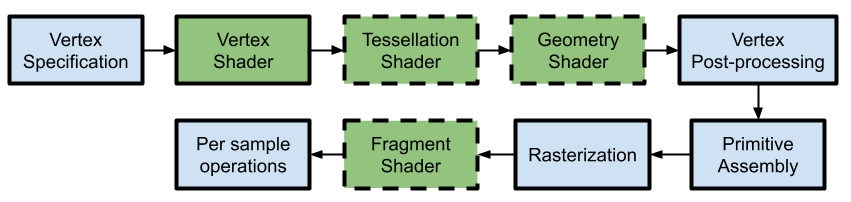
\includegraphics[width=0.7\textwidth]{img/RenderPipeline}
\end{figure} 
\end{frame}

\begin{frame}{Simplificando\ldots}
\begin{itemize}
    \item El la práctica, los tesselation shaders y los geometry shaders solo se usan para cosas muy especificas.
    \item Mas aún, casi nunca se configuran los estados entre el vertex shader y la rasterización
    \item Para propósitos de esta explicación, podemos pensarlo de manera mas simple:    
\end{itemize}
\begin{figure}[htb]
  \centering
  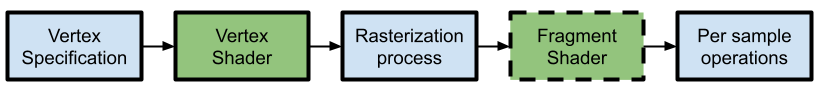
\includegraphics[width=0.7\textwidth]{img/SimplifiedPipeline}
\end{figure}
\end{frame}

\begin{frame}[allowframebreaks]{¿Cómo se programa una aplicación gráfica?}
\begin{itemize}
    \item En general tienes que usar al menos tres cosas:
    \begin{enumerate}
        \item Un lenguaje de programación del lado del CPU para crear una aplicación.
        \item Un API gráfico, para construir, configurar y conectar el pipeline.
        \item Un lenguaje para escribir shaders.
    \end{enumerate}
    \item En este taller solo escribiremos código de shaders usando \href{https://www.khronos.org/opengl/wiki/OpenGL_Shading_Language}{GLSL}.
    \item Pero sin darnos cuenta el navegador de hecho usa: \href{https://en.wikipedia.org/wiki/JavaScript}{javascript} y \href{https://www.khronos.org/webgl/}{WebGL}, que es un \href{https://www.khronos.org/opengles/}{subconjunto de OpenGL}.
\end{itemize}
\begin{figure}[htb]
  \centering
  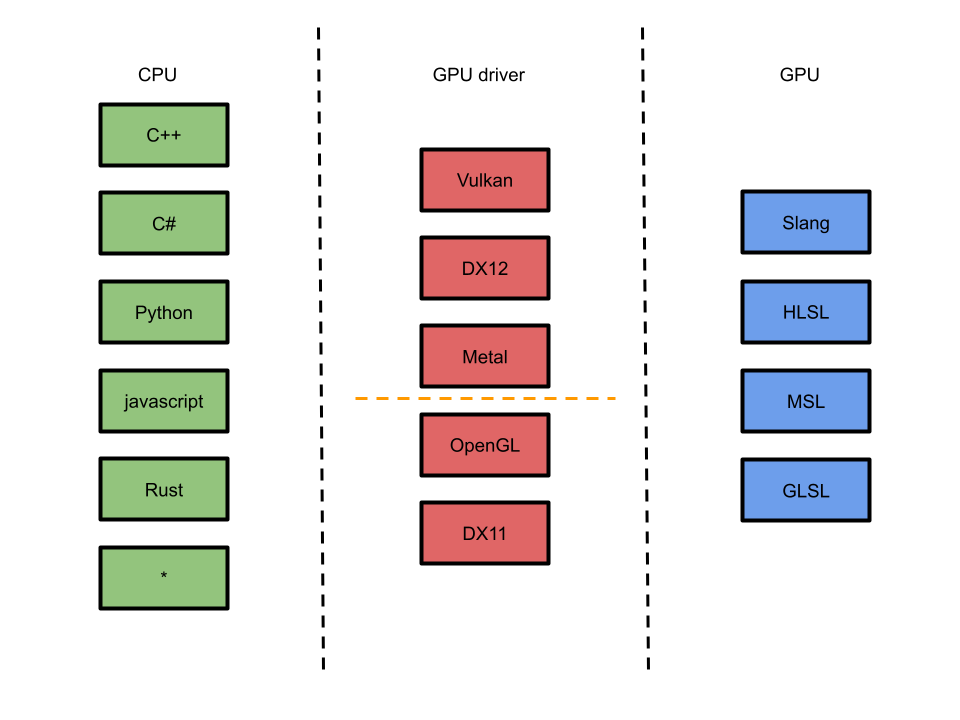
\includegraphics[width=0.6\textwidth]{img/APIs}
  %\caption{Hay varias opciones para cada caso}
\end{figure}
\end{frame}

\begin{frame}[allowframebreaks]{Anatomía de una aplicación}
Actualmente, una aplicación típica:
    \begin{itemize}
        \item Esta escrita en un engine gráfico (Como \href{https://unity.com/}{Unity} o \href{https://www.unrealengine.com/}{Unreal})
        \item Para producir un frame, se usan cientos de pipelines.
        \begin{itemize}
            \item Varios pipelines, producen resultados en texturas que luego otros pipelines consumen
            \item Cada material de los objetos de la escena tiene su propio pipeline
            \item Hay pipelines especializados en ciertas tareas (Sombras, reflexiones, iluminación, etc.)
            \item Algunos son directos, otros diferidos, otros por mosaicos
            \item Sin contar que muchos efectos se llevan a cabo en compute shaders
        \end{itemize}
    \end{itemize}
    \begin{figure}[htb]
        \centering
        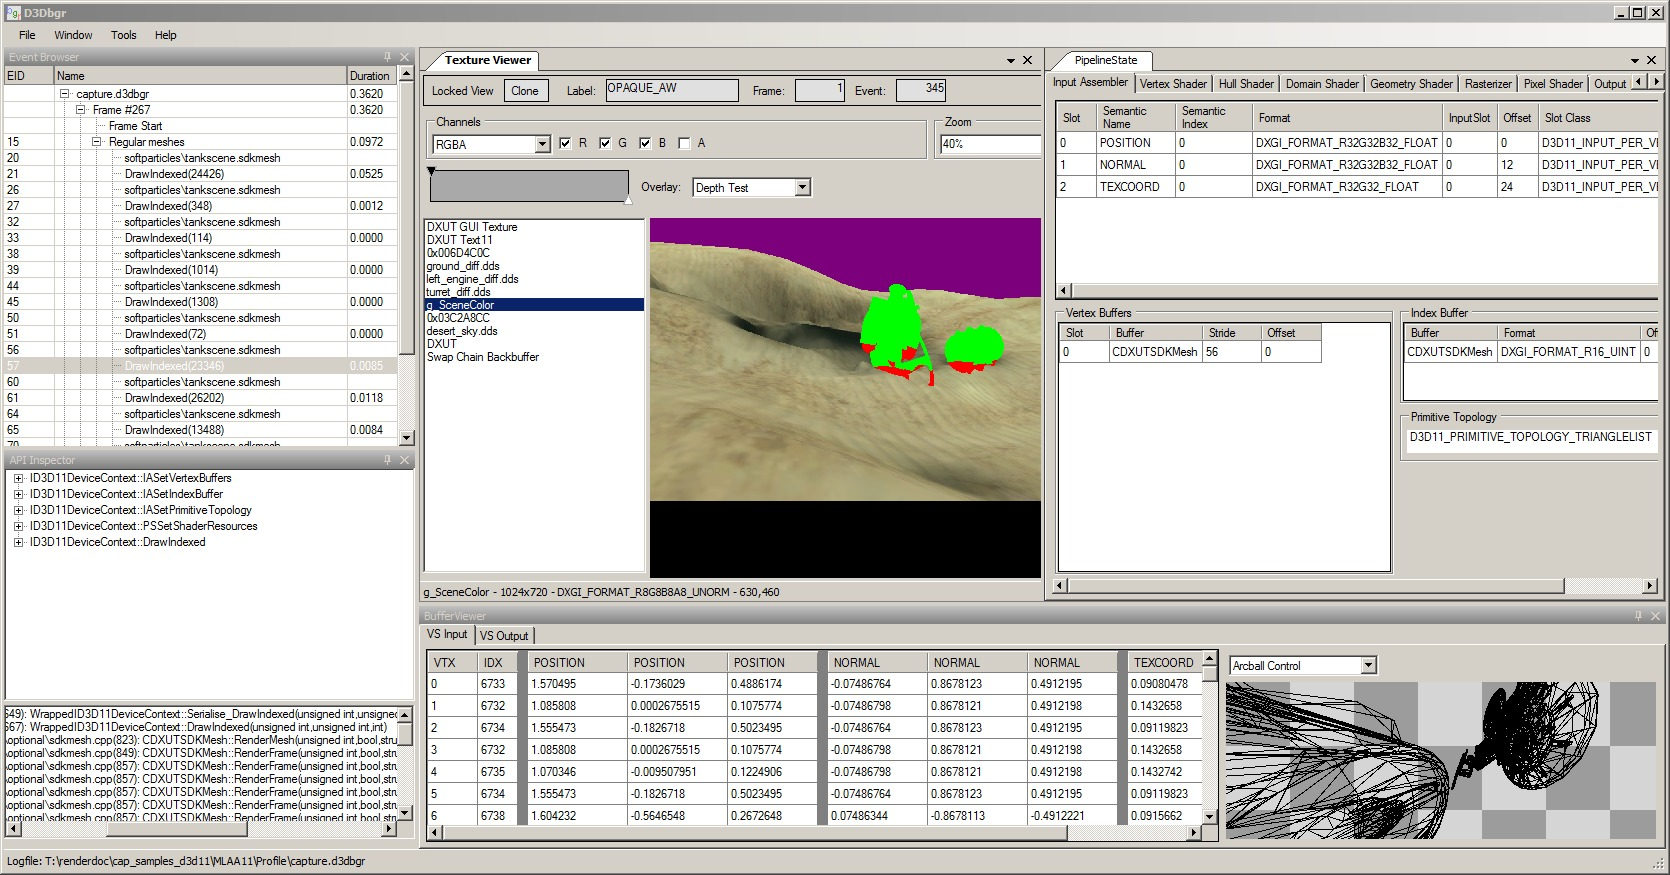
\includegraphics[width=0.8\textwidth]{img/functionality}
    \end{figure}
\end{frame}

\begin{frame}{¿Qué nos depara el futuro?}
\begin{columns}
\column[t]{0.5\textwidth}
    Hay una tendencia importante hacia:
    \begin{itemize}
        \item Unificar en el modelo de \href{https://en.wikipedia.org/wiki/Physically_based_rendering}{iluminación PBR}
        \item Las técnicas basadas en rayos: \href{https://en.wikipedia.org/wiki/Ray_tracing_(graphics)}{Raytracer}, \href{https://en.wikipedia.org/wiki/Ray_marching}{Raymarching}, \href{https://en.wikipedia.org/wiki/Path_tracing}{Pathtracers}
        \begin{itemize}
            \item Generar parte de los fragments de un frame, \href{https://www.youtube.com/watch?v=5PHBXY0FI5o&t=2s}{usando técnicas de AI} en vez de calcularlos
        \end{itemize}
        \item Definir un nuevo pipeline: Task (Amplification) shaders, \href{https://www.khronos.org/blog/mesh-shading-for-vulkan}{mesh shaders}
        \item Descargar la mayor parte de la tareas en el \href{https://en.wikipedia.org/wiki/Compute_kernel}{compute shader}
    \end{itemize}
\column[t]{0.5\textwidth}
\begin{figure}[htp]
  \centering
  \includegraphics[width=0.6\textwidth]{img/pathtracer}
\end{figure}
\end{columns}
\end{frame}

